\chapter{Conceptual Design}\label{Ch3}
In this chapter, a conceptual design of the Body Temperature Measuring Wristband will be presented. The Model-Based Systems Engineering, or MBSE, process will be followed during the design. The MBSE model should not be confused with a mathematical- or simulation model but instead as a conceptual model. The system as a whole will be viewed on a high level, where-after it will be broken down into more detailed levels. A Functional Analysis of the system will be used to determine how the system will monitor and display body temperature, after which an Architectural Synthesis will determine with what functional elements this could be accomplished. After completion of the Functional Analysis, and the Architectural Synthesis, Resource Allocation matrices will be used to test if the design is valid. This chapter will only show the design on a concept level, the detailed design will follow in subsequent chapters. 

\section{Functional Analysis}
Functional analysis is a tool to describe the behaviour of the system on a lower level. Functional analysis does not determine or state how a specific function is accomplished, just that it needs to be accomplished. Therefore, the purpose of functional analysis is to identify and clearly state how the system is to work when fully completed. The functional flow block diagrams used in functional analysis uses a level type hierarchy where the system functions are expanded from a high level (level 0) to a lower level, consisting of more detail.  

\subsection{Level 0}
The functional analysis is started at the system life cycle, which is also level 0 of the functional flow diagram. Level 0 of the functional flow diagram shows the very high level functions of the system at any point in time. The level 0 functional flow diagram of the system is shown in \autoref{fig:9}.
\begin{figure}[H]
	\centering
	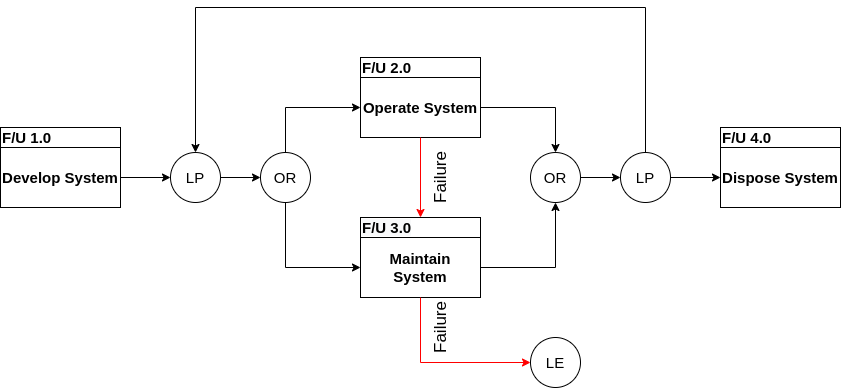
\includegraphics[scale=0.5]{img/L0FF}
	\caption{Level 0 Functional Flow}
	\label{fig:9}
\end{figure}
\noindent
The system will mostly be in the Operate System function seen in \autoref{fig:9}. Once a failure occurs in this state, the system will transition to the Maintain System function. If an unrepairable error occurs, the system will exit the loop and the system will be disposed of.  

\subsection{Level 1}
The level 1 functional flow diagram provides further detail on how the system functions. The blocks from level 0 are expanded to provide more context on that function of the system. The level 1 functional flow of the system is shown in \autoref{fig:10}.
\begin{figure}[H]
	\centering
	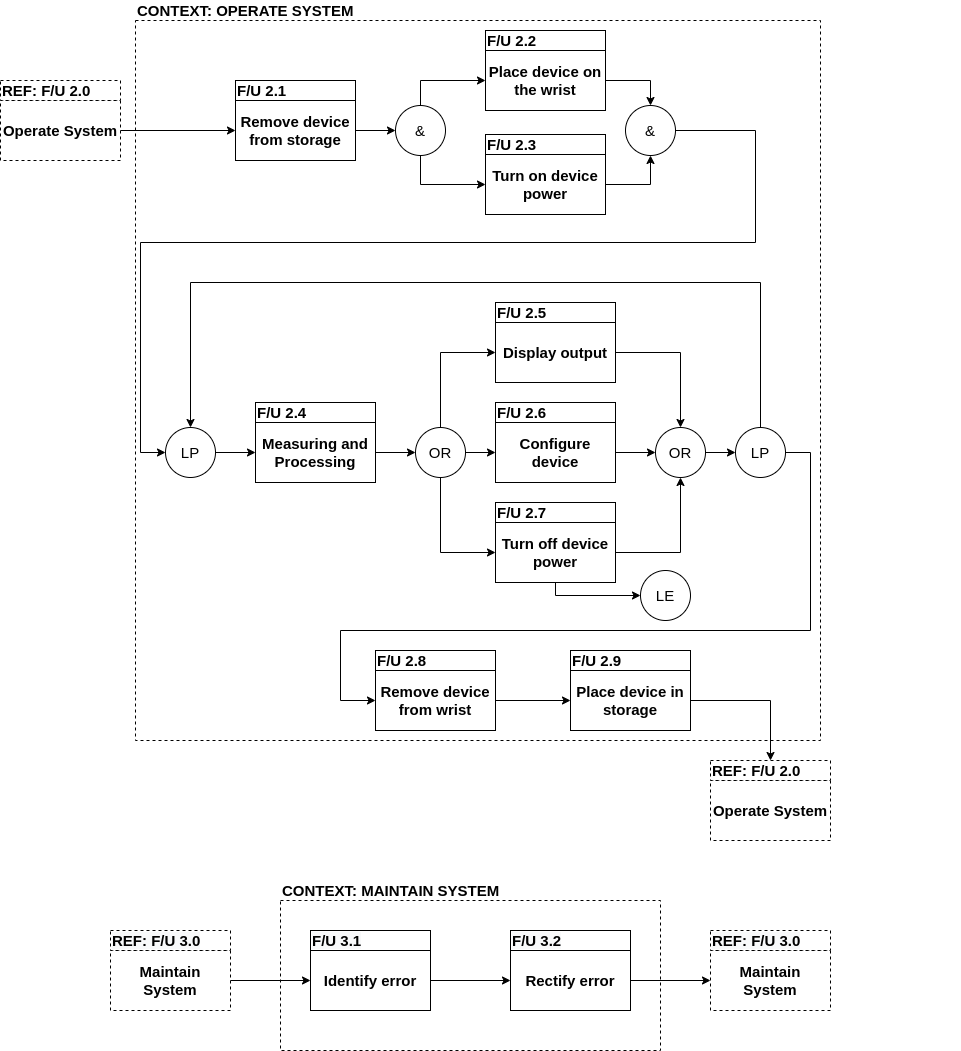
\includegraphics[scale=0.5]{img/L1FF}
	\caption{Level 1 Functional Flow}
	\label{fig:10}
\end{figure}
\noindent
The Operate- and Maintain System functions are expanded in level 1 of the functional flow diagram, and more detailed functions within each are revealed. Some of the blocks in level 1 of the functional flow diagram can be expanded even more. 

\subsection{Level 2}
Level 2 of the functional flow diagram is the in-depth investigation of the blocks from level 1 that can be expanded further. More information on how the system is to function can be seen in level 2 of the functional flow diagram. Blocks from the Operate System context found in \autoref{fig:10}, that can be expanded further are shown in \autoref{fig:11} and \autoref{fig:12}.
\begin{figure}[H]
	\centering
	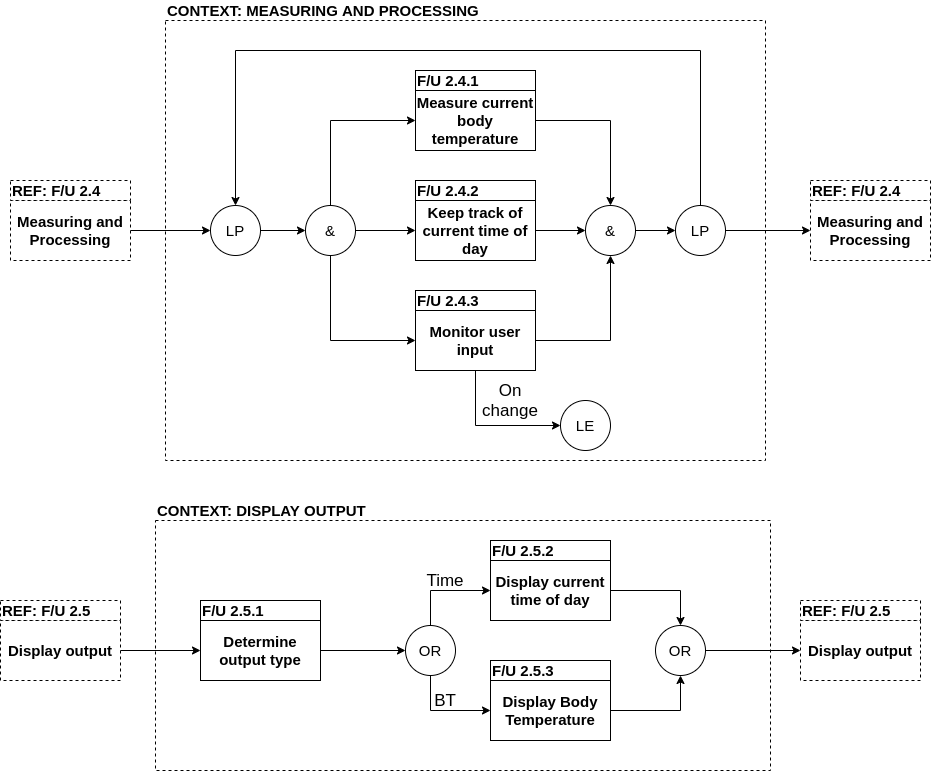
\includegraphics[scale=0.5]{img/L2FF1}
	\caption{Level 2 Functional Flow - Operate System Part 1}
	\label{fig:11}
\end{figure}
\noindent
From \autoref{fig:10} and \autoref{fig:11}, it is clear that the system will mostly be in the Measuring and Processing state where the current body temperature of the user will be measured and general timekeeping will be performed. The system will only go to the next function, which is to display certain information to the user, if prompted. After the system has displayed the requested information, it will return to the Measuring and Processing state. Note, however, that general timekeeping will always be performed by the system, no matter the current function. If the user requests to see the current time of day or current body temperature, the applicable output will be shown.
\begin{figure}[H]
	\centering
	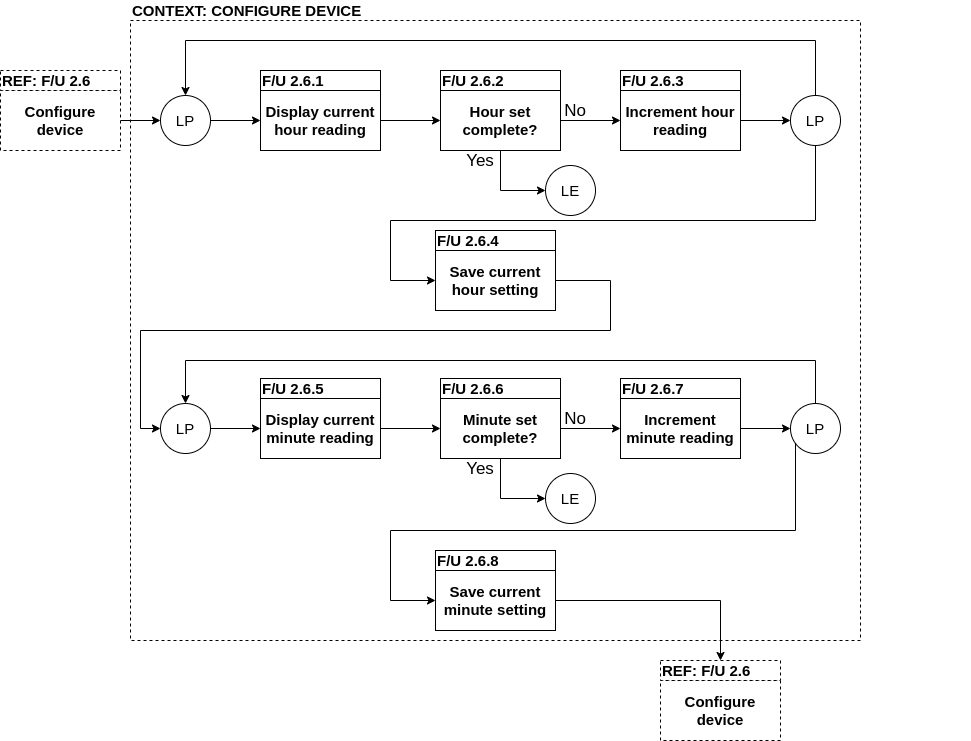
\includegraphics[scale=0.5]{img/L2FF2}
	\caption{Level 2 Functional Flow - Operate System Part 2}
	\label{fig:12}
\end{figure}
\noindent
Once the user requests to configure the device, the current time of day can be set correctly. The process can be seen in \autoref{fig:12}, where the current saved hour reading is shown to the user, this hour reading will be incremented until the user finds it suitable. The hour reading will then be saved. The same process holds for setting the minute reading. 
\\
\\
Blocks from the Maintain System context found in \autoref{fig:10}, that can be expanded further are shown in \autoref{fig:13}.
\begin{figure}[H]
	\centering
	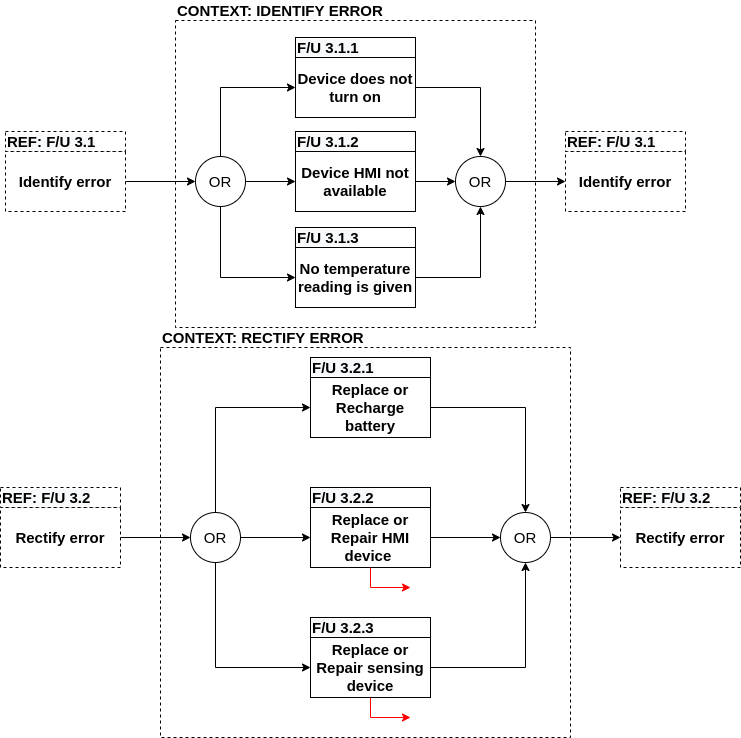
\includegraphics[scale=0.5]{img/L2FF3}
	\caption{Level 2 Functional Flow - Maintain System}
	\label{fig:13}
\end{figure}
\noindent
The Identify error and Rectify error functions from the Maintain System functional diagram are used to find the origin of the error, as well as to rectify the error. If the error is not repairable, the system will transition to the Dispose System state, as mentioned earlier. 

\section{Architectural Synthesis}
Architectural Synthesis is also known as Physical Design and is a process by which the design, that has been captured up to this point in the Functional Analysis, is transformed into something that can be constructed on a concept level. Architectural Synthesis is used to determine what functional elements, or resources, are needed by the system to be able to accomplish the functions mentioned in the previous section. Architectural Synthesis, once again, follows the same level type hierarchy as with the Functional Analysis. In this process, the functional flow elements will be mapped to the physical architecture of the system. 

\subsection{Level 0}
The high level physical architecture of the system is shown in \autoref{fig:14}. At this level, the different objects the system will interact with, denoted as functional units, are seen. 
\begin{figure}[H]
	\centering
	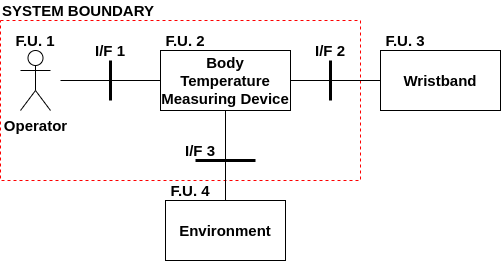
\includegraphics[scale=0.5]{img/L0PA}
	\caption{Level 0 Physical Architecture}
	\label{fig:14}
\end{figure}
\noindent
The system boundary clearly shows the system that will be designed, and the operator or user that will be using the system. Functional Unit 2, which is the Body Temperature Measuring Device is the system of interest, and the Physical Architecture of this unit will be expanded in the level to follow, to show the resources needed to design and construct the system. 

\subsection{Level 1}
The expansion of the Body Temperature Measuring Device from level 0 are shown in \autoref{fig:15}.
\begin{figure}[H]
	\centering
	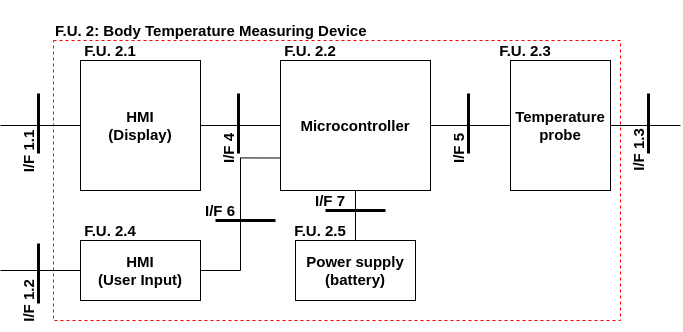
\includegraphics[scale=0.5]{img/L1PA}
	\caption{Level 1 Physical Architecture}
	\label{fig:15}
\end{figure}
\noindent
From \autoref{fig:15} the physical resources needed to implement the system can be seen, as well as how these resources interface with each other and the outside world.
This is the Physical Architecture that will be used in the detailed design of the system, where specific components will be assigned to each resource. 

\section{Resource Allocation}
Resource Allocation matrices are used to test if the conceptual design is valid. A resource allocation matrix compares the available resources to the functions that needs to be performed. Therefore, the functions from the Functional Analysis are compared to the resources from the Architectural Analysis, to see if there is a resource available to perform the specific function, and vice versa. 
\\
\\
The resource allocation matrix that compares the high level functions to the high level resources are shown in \autoref{fig:16}.
\begin{figure}[H]
	\centering
	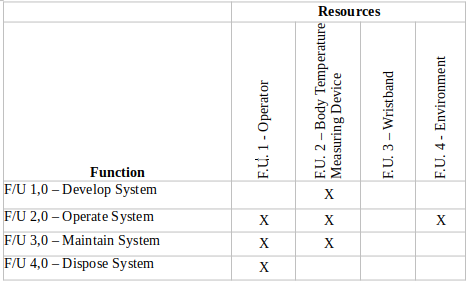
\includegraphics[scale=0.6]{img/RA0}
	\caption{High level Resource Allocation matix}
	\label{fig:16}
\end{figure}
\noindent
The resource allocation matrix that compares the lower level functions to the lower level resources are shown in \autoref{fig:17}.
\begin{figure}[H]
	\centering
	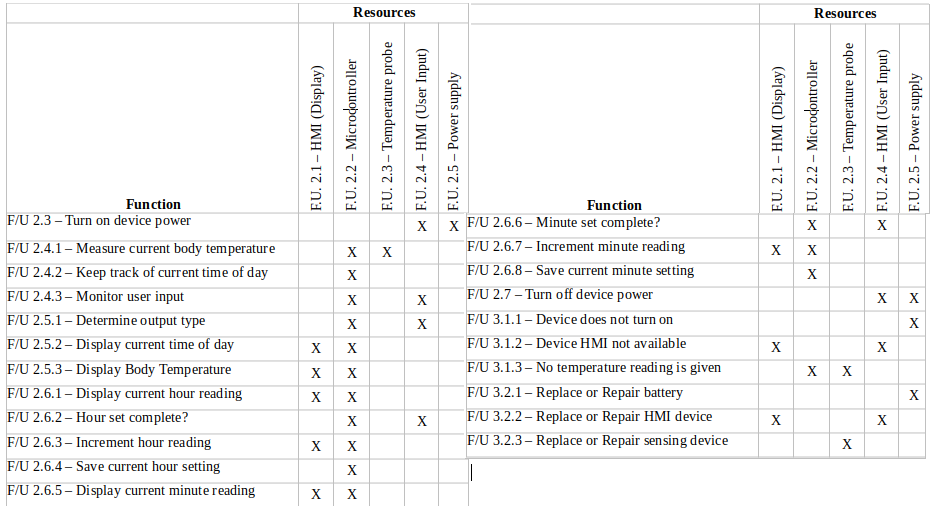
\includegraphics[scale=0.5]{img/RA2}
	\caption{Lower level Resource Allocation matix}
	\label{fig:17}
\end{figure}
\noindent
From the resource allocation matrices it is clear that the concept design is feasible and valid since there are no functions that are not allocated to a resource, and no resources not being used by any functions.

\section{Concluding Remarks}
This section showed the process followed in the concept design of the Medical Wristband Body Temperature Monitor. A Functional Analysis was used to clearly state how the system is to work when fully deployed. After this, an Architectural Synthesis was used to determine the physical architecture of the system, and what resources are available to perform the functions from the Functional Analysis. Finally, Resource Allocation matrices were used for the validation of the concept design. 